%!TEX root = ../Peerbox.tex

As illustrated in Figure~\ref{fig:figures_archOverview} the Peerbox client is structured according to the layered approach. The Middleware layer is concerned about the low level network communication. The Logic layer provides the functionality for the VirtualFileSystem and contains the application logic. The UI represents the user layer and provides the functionality for user interaction.

\begin{figure}[htbp]
    \centering
        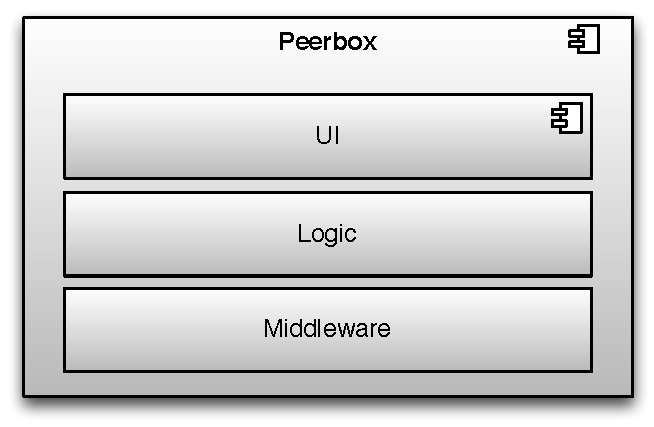
\includegraphics[height=2in]{figures/archOverview.pdf}
    \caption{Architectural overview}
    \label{fig:figures_archOverview}
\end{figure}

We have decided to use two different channels for communication. The general Peerbox related communication uses multicast message while file transmission is implemented by using a 1-1 direct channel. 
The reason for this is that files are arbitrary large and would produce a lot of messages that need to be multicasted. Furthermore, not all clients might be interested in every file. Last but not the least, a direct channel is fast and reliable as we can rely on the build-in properties of the TCP/IP protocol.

Peerbox has been implemented in Java 7 and uses the following third party libraries: 
\begin{itemize}
    \item Apache Commons Lang, for timed semaphore
    \item Apache Log4j, for general purpose logging
    \item Apache Commons IO, log file tailing
    \item SWT, user interface
\end{itemize}

\subsection{Middleware}

The middleware of peerbox uses IP-Multicast to announce messages to a group. However, basic multicast is not reliable and it does not ensure integrity, validity, agreement and ordering.

A test implementation of using the IP multicast showed a package loss of up to 20\% depending on the operating system, hardware and message frequency. 
Therefore, we need additional coordination and agreements on message receiving and delivery in the form of a reliable multicast protocol.

% open vs. closed group 
%  only members can send to group, a member delivers to itself 
%  they are useful for coordination of groups of cooperating servers

The multicast protocol should ensure that all messages send to a group are eventually received and consumed by all process that are member of this group. Furthermore, messages need to be consumed in order, so that a file cannot be deleted before it has been created. 

For peerbox it is enough to ensure FIFO-ordering. Since a file always has a specific owner, it is enough if the messages from one process are consumed in order and are independent from another processes (no causality required). 

We implemented the reliable multicast based on the lecture slides, using  piggybacked messages number, negative acknowledgement and a holdback queue. Furthermore, we optimized the implementation using  multi-threading, bandwidth limiting, checksum and send optimizations. 
    
In the following sections, we will use the following terminology. Multicast a message means to send a message to a multicast group. Receiving a message means that a message has been received from a multicast group but has not yet been forwarded to the application logic. For example, as it has not arrived in the correct order. Delivering a message from group g means that the message has been received in correct order and can be consumed by the application logic.


% % The IP address 224.0.0.0 through 239.255.255.255 are reserved for multicasts. The user needs to set some properties such as Path, Multicast address, Multicast port, Server Port and the name of the computer.
 
% over udp datagram
% 
% negative acknowledgements
% 
% reliable multicast
% 
% additional checksum to verify payload
% 
% Operations 
% multicast(g, m) sends message m to all members of process group g
% deliver (m) is called to get a multicast message delivered. It is different 
% from receive as it may be delayed to allow for ordering or reliability.

\subsubsection{Messages}
The basic entity of our reliable multicast implementation is a Message, whose structure is shown in Figure~\ref{fig:messages}. The first byte represents the command, hence the message supports $2^8$ different commands. In our case, a command can be either Message (1), ACK(2), NACK(4), or HEARTBEAT(8). However, ACK messages are not used in this implementation in order to reduce traffic on the channel. Furthermore, the peer and message number are represented each by four bytes. Afterwards, the length of the payload is specified by two bytes. Eight bytes are reserved for the checksum, which is calculated on the payload using a Cyclic Redundancy Check (CRC32). The actual payload has no fixed size and is only limited by the maximum message size, which is in our case is set to $2^{15}$.

If the logic layer needs to send a lot of data, it has to be split into multiple messages. Due to the reliable multicast, it is guaranteed that all messages will eventually arrive and are consumed in order.

\begin{figure}[htbp]
    \centering
        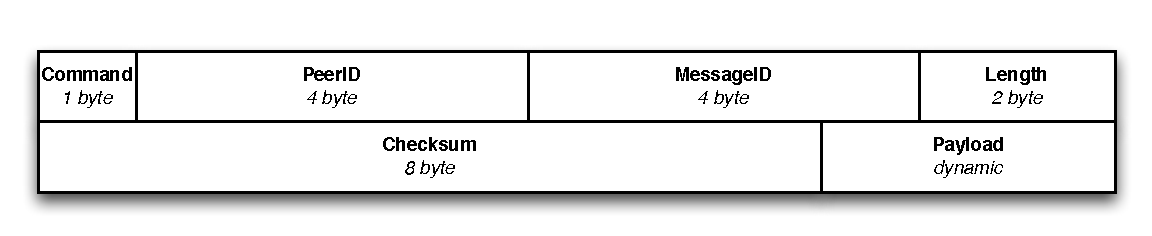
\includegraphics[width=.9\textwidth]{figures/message.pdf}
    \caption{Structure of a message}
    \label{fig:messages}
\end{figure}

\subsubsection{Delivering Messages from the Group}
Figure~\ref{fig:figures_processReceivePackage} shows the process view on the activity of listening for incoming messages and processing those messages. The actual consumption and reliability processes is shown in Figure~\ref{fig:figures_processMessages}.
The use of resources  is indicated by a dashed line 
processes are divided by swim-lanes (dotted vertical lines)
\begin{figure}[htbp]
    \centering
        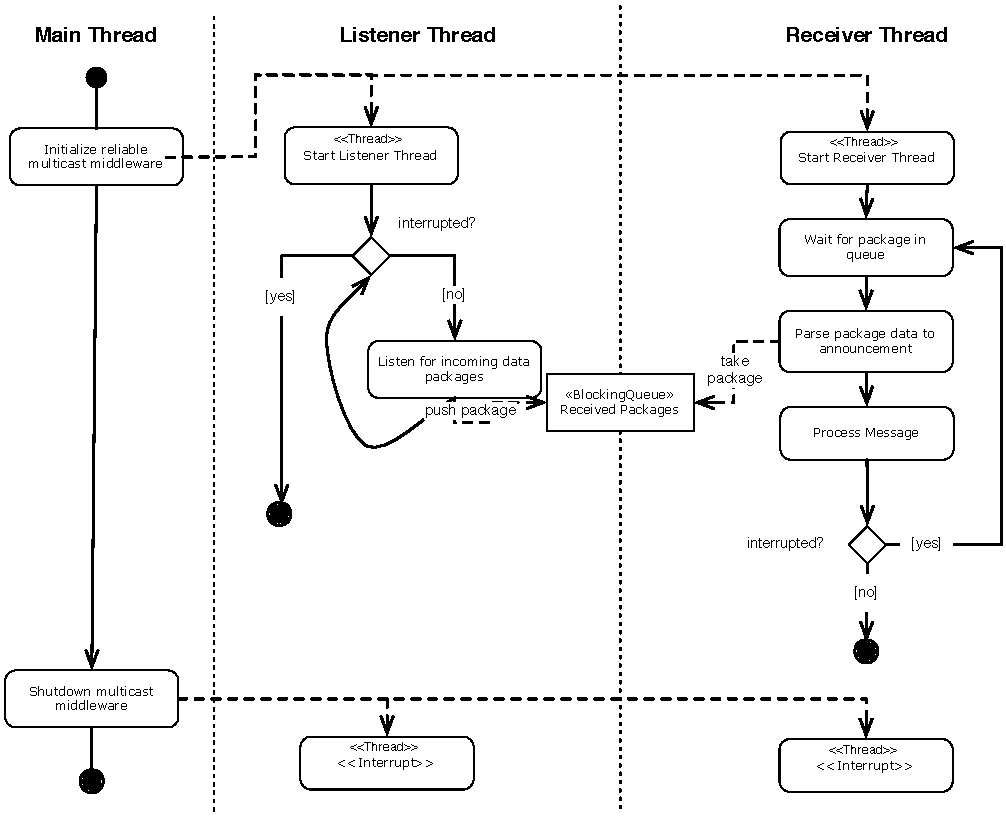
\includegraphics[height=4.5in]{figures/receivePackets.pdf}
    \caption{Listen for incoming multicast messages}
    \label{fig:figures_processReceivePackage}
\end{figure}
When the middleware is initialized it starts separate listener threads and a received thread. The listener waits incoming messages on the channel of the multicast group. as soon as it receives a message, it pushes it on a blocking queue for received packages and immediately continues to listen for the next message. 

Listening and processing of incoming messages has been decoupled by a blocking queue to decouple lengthy processing from receiving new messages, if the blocking queue is full, the listener thread has to wait until all packets have been processed. 

On the other side, the receiver thread takes packets from the blocking queue and processes them. If the queue is empty,  it waits until the listener thread has received and pushes the next package. 
At first the receiver thread parses the incoming packet into the aforementioned message structure and then decides wether the message is directly consumed, discarded or pushed on to the holdback queue for later consumption.

This process is described in Figure~\ref{fig:figures_processMessages}.
Depending on the command of the message, the message either contains data or is a request for a missed message (Nack). If it is a NACK,  then the process resends the requested message by taking it from the sent messages list.



If the command is actually a message it first checks, whether it has ever received a message from that particular process before. If not, it initializes the piggyback counter and set the seen message id to the id of the current received message minus one.

Every peer holds the id of every other peer, that is member of the group, a piggyback counter that contains the id of the last consumed message from that peer and the id of the last seen message, ideally both are the same.
Afterwards, it compares the local piggyback counter with the piggybacked messages number. One of three things might happen. 

1) The message has been seen before and is discarded.
2) The message id is larger than the expected message, which means that a message has been missed. A negative acknowledge is sent for the missed message. 
3) The message is expected and can be reliably consumed, which involves another multicast of the message to the group.
 
\begin{figure}[htbp]
    \centering
        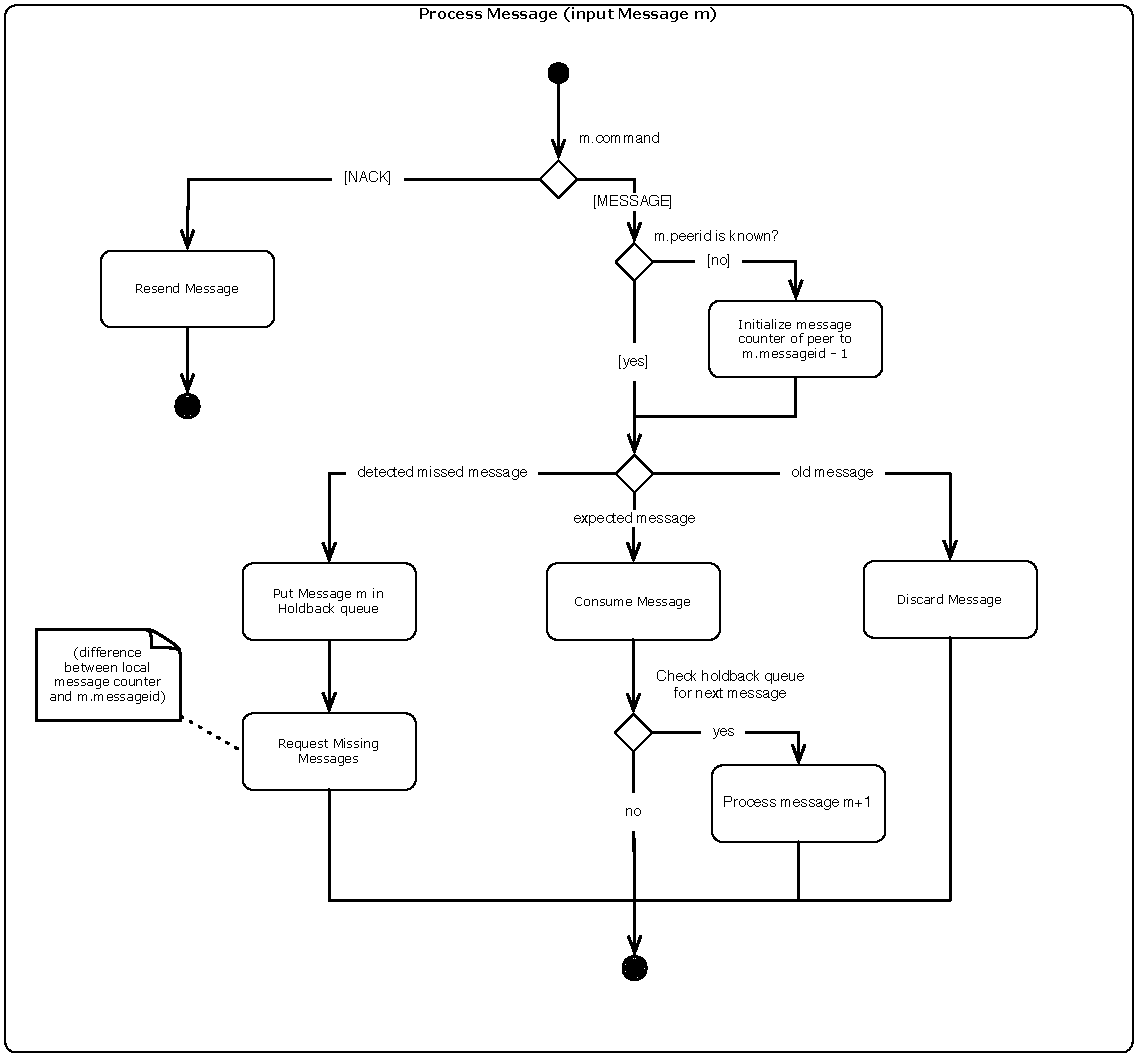
\includegraphics[height=4.5in]{figures/processMessages.pdf}
    \caption{Process incoming multicast messages}
    \label{fig:figures_processMessages}
\end{figure}

\subsubsection{Sending Messages to the group}

The process of multicasting a message to the group is described in Figure~\ref{fig:sendMessage}. Sending a message to a group is quite simple and easy in Java. At first the message will be serialized into an array of bytes, which will be multicasted by using the Socket class. 

However, we have implemented various optimizations in order to improve reliability and to avoid clogging of the network. For instance, we figured out that if we limit the frequency of messages, less messages are lost. This is similar to limiting the bandwidth because less bits per seconds can be transferred.  
We implemented the limit by using a timed semaphore, which ensures that a critical path can only be entered in every given time frame. Since Peerbox is not time critical, it is not a  problem to limit the bandwidth. 
However, the timed semaphore is not enough because this will cause the application to halt until it can enter the critical section. Therefore, we decoupled  sending from the main application by using a blocking queue, which acts as a send buffer. 

To summarize, the sender thread tries to acquire the semaphores, takes the next message from the queue, multicasts it to the group and then waits again for the semaphore and the next message. 

Furthermore, the send buffer allows to reduce the amount of sent messages by discarding messages that are already in the send buffer but are not yet  multicasted to the group. Therefore, before pushing a message to the send buffer, it is checked if the message is already present in the buffer.
An analysis of the network traffic showed that a lot of negative acknowledgements were sent multiple times because the process encountered a missed message multiple times. However, this process did not have the chance to multicast the first negative acknowledgement.

\begin{figure}[htbp]
    \centering
        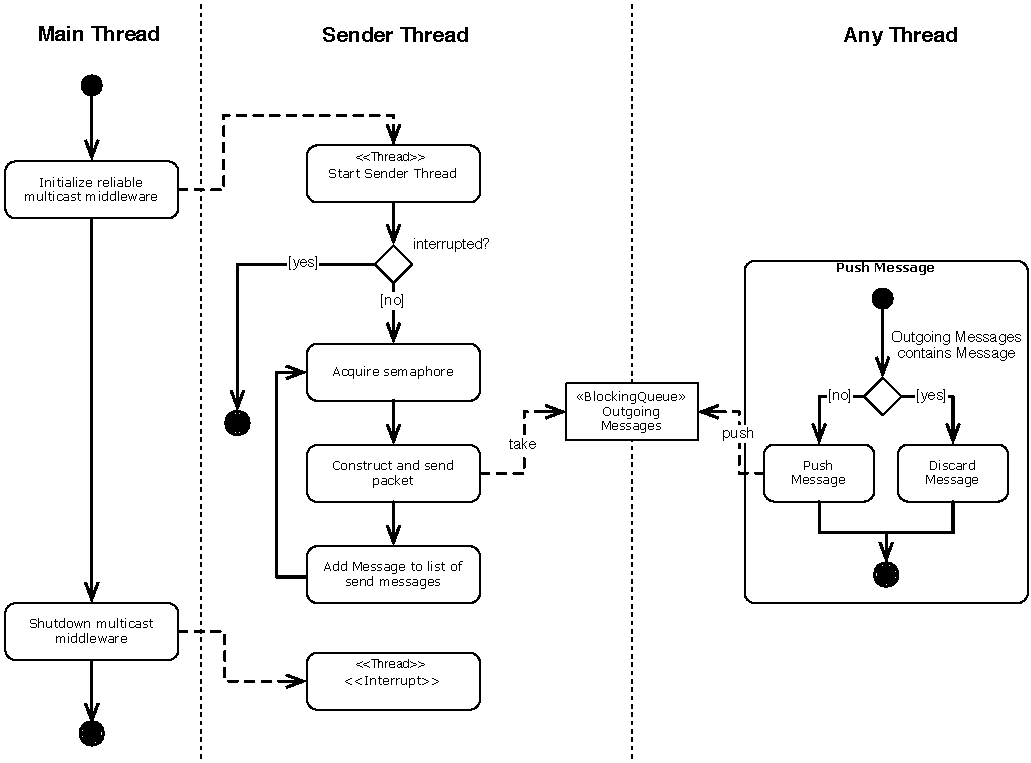
\includegraphics[height=3in]{figures/sendMessage.pdf}
    \caption{Send a multicast message}
    \label{fig:sendMessage}
\end{figure}
  
\subsubsection{Hearbeat}
A tough challenge is to handle peers that leave without notice. Firstly, it is difficult to distinguish between a crashed peer or a slow peer and  secondly there is no automatic mechanism implemented in the basic multicast that informs other peers if a peer leaves the group.

We consider two tactics to increase fault-tolerance. The first one is a ping-echo tactic, in which a peer sends a ping message to another peer. If the peer answers with an echo message, everything is fine if not, the peer is down for the count. We tried to implement the ping-echo mechanism using a reliable 1-1 channel, i.e. TCP/IP. In order to reduce the number of ping/echo messages, it would be good to have one peer that is responsible for sending out pings and detecting dead peers. This would require a leader-election algorithm.

The alternative is a heartbeat tactic, in which every peer multicasts a life signal in a certain time interval. The dead peer detection is done by every peer on its own. Although the multicasted heartbeat might be less reliable as a fault-detection algorithm because it might happen that peers are in a different state (e.g. if one peer misses heartbeat messages), the complexity and total amount of messages is lower compared to the described ping/echo tactic.

Therefore, we implement a heartbeat mechanism into the middleware to be able to detect unresponsive peers.

\subsubsection{Optimizations}
The following optimizations have been implemented or were considered for implementation.

When a peer p detects that it has missed a message m from peer q, it will send a negative acknowledgment. However, if the negative acknowledgment or the resend message is lost, the peer p will not ask again for that message until it receives another message from peer q. 
In the Peerbox system, the time frame between two messages could be arbitrarily large, which means that a peer might wait for a long period until he finally receives and consumes a message. 
By associating a negative acknowledgement with a timer, the peer will automatically send the negative acknowledgement again if it has not yet received the message.

Another optimization would be to dynamically limit the bandwidth based on heuristics. For example, if the number of messages and peers increase a certain threshold, the bandwidth can be reduced by increasing the time frame of the semaphore. 

Causal ordering can be implemented by using vector clocks. The vector clock of a peer p is piggybacked to message m. A peer q, which receives m is only allowed to deliver m, if it has seen all messages that p has seen. Otherwise,it can send negative acknowledgements based on the vector clock of p. 

\subsection{Logic}
The application logic is mainly responsible for processing dispatched messages from the middleware and maintains a consistent Virtual File System.
    
\subsubsection{Messages}   
The actual Peerbox messages are stacked on the Multicast Messages of the middleware which means that they will be serialized into the payload of a multicast message. 
Instead of using a predetermined structure, we decided to use a more open-approach that allows for easy modifiability and an simple extension of the protocol. Hence, we are using a Key-Value store, which will be serialized and deserialized. 

The actual type of a message is defined by the Key command, which might contain one of the following values illustrated in Listing~\ref{lst:keyvalues}. In concrete, we use the HashMap class, which can be easily serialized using Java serialization API.  The HashMap takes objects of the enum-type Key as keys and any type of Object as value. The application logic is responsible to cast the value to the appropriate type, e.g. \verb|Command c = (Command)message.get(Key.Command);|.

\begin{lstlisting}[caption=Possible values of command, label=lst:keyvalues]
public static interface Command {
		public enum Request {
			List, Join, Token;
		}

		public enum Reply {
			List, Welcome, Token;
		}

		public enum Info {
			Created, Deleted, Modified, Leave;
		}
	}
\end{lstlisting}

\subsubsection{Message handling}
Due to the diversity of messages that are sent in the logic layer, the Strategy Pattern has been implemented to execute the appropriate algorithm depending on the received Key.Command. The Strategy is implemented by an abstract MessageHandler class, which provides a static method to process a message. The process method that forwards the message to the appropriate concrete MessageHandler, e.g. ReplyListMessageHandler which multicast a list of local files. The concrete messages and the actual creation of the VirtualFileSystem will be described in the following section. 

Using the StrategyPattern increases the cohesion and thus improves maintainability, because MessageHandler have a concrete task and new MessageHandler can be easily added.

\begin{figure}[htbp]
\centering
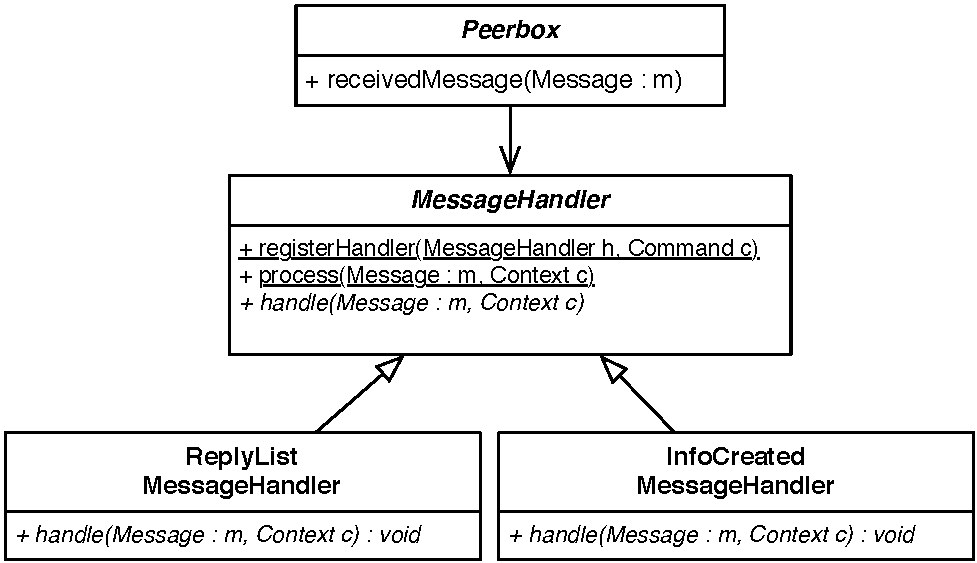
\includegraphics[height=2in]{figures/mhStrategy.pdf}
\caption{Strategy Pattern for handling messages}
\label{fig:figures_mhStrategy}
\end{figure}


\subsubsection{Virtual File System}
    
The \gls{acr:vfs} contains a File List which is a dictionary of \glspl{acr:ufid} and Peerbox Files. We decided to create our own entity in order to represent a file, instead of using the Java File entity. We did this in order to create a virtual file which contains only the important information and not the data. Furthermore, the Java File entity contains operating system specific information that should not be shared with the rest of the peers. The Peerbox Files are associated with peers. This means that File List could contain two files with the same file name belonging to different peers.
    
The VFS is responsible for maintaining the consistency of the File List among all peers. This is mainly accomplished with two techniques. The first one by observing the local file system for changes, e.g. file creations, deletions, or modifications, and updating the local File List. The second one is to multicast these changes to the rest of the peers so they can also update their own local File Lists.

The current implementation of Peerbox does not allow the creation, deletion, and updating of remote files. This can be accomplished by introducing a token-based approach. Each token is paired with a file and denotes the owner of the file. Ownership can change when a peer agrees to give the token of a particular file to another peer. In this way peers would be able to apply changes to a remote File System.

The VFS has some limitations. The most important of them is the fact that there is no real file system shared between peers. Hence, it is possible to invalidate the state of the VFS by modifying the Peerbox folder when the application is not running.

\subsubsection{Dynamicity}
Since Peerbox will be used on different operating systems and changing environments, it is important that it allows for a certain configuration dynamicity. Therefore, it tries to dynamically configure itself whenever possible, e.g. it dynamically receives the IP-Address and port from remote peers or it obtains the folder and username from the system properties. If a dynamic approach is not possible, the configuration options are at least configurable via a property file. 
For example, it is possible to specify the Multicast-address and port.

\subsection{Interface}
The focus of this report lies on the implementation of the distributed aspects of Peerbox. Nevertheless, in order to use the system a simple user interface has been implemented using the Simple Widget Toolkit (SWT) and a Model-View-Controller approach. The user interface is shown in Figure~\ref{fig:figures_gui}.
\begin{figure}[htbp]
    \centering
        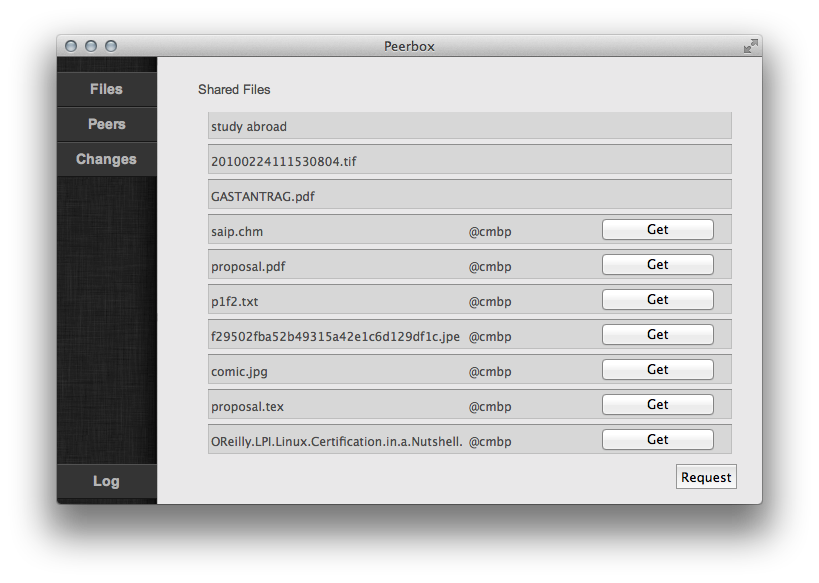
\includegraphics[height=4.15in]{figures/gui.png}
    \caption{User interface}
    \label{fig:figures_gui}
\end{figure}
